\documentclass[12pt]{article}
\usepackage[margin=1in]{geometry}
\usepackage[T1]{fontenc}
\usepackage{mathptmx}
\usepackage[parfill]{parskip}
%\usepackage{amsmath}
\usepackage{graphicx}
%\usepackage{listings}   % allows lstlisting environment
%\usepackage{moreverb}   % allows listinginput environment
%\usepackage{siunitx}
%\usepackage{enumerate}
%\usepackage{epstopdf}
%\usepackage{booktabs}
%\usepackage{float}
%\usepackage{multirow}
%\usepackage{mhchem}
%\usepackage{lscape}
\usepackage{hyperref}
\hypersetup{
    colorlinks=true,
    linkcolor=blue,
    filecolor=magenta,      
    urlcolor=cyan,
}

\newcommand{\horrule}[1]{\rule{\linewidth}{#1}} % Create horizontal rule command with 1 argument of height

\newcommand\mytitle{Evolution 2\\Compsci 458}
\title{\horrule{5pt}\\\vspace{0.4cm}{\bf \mytitle}\\}
\author{Jiawei Zhang, Davis Treybig, Michael Han, and Kevin Do}
\date{\horrule{1pt}}

\begin{document}
\maketitle{}
\section{Summary}
\begin{figure}[h]
\begin{center}
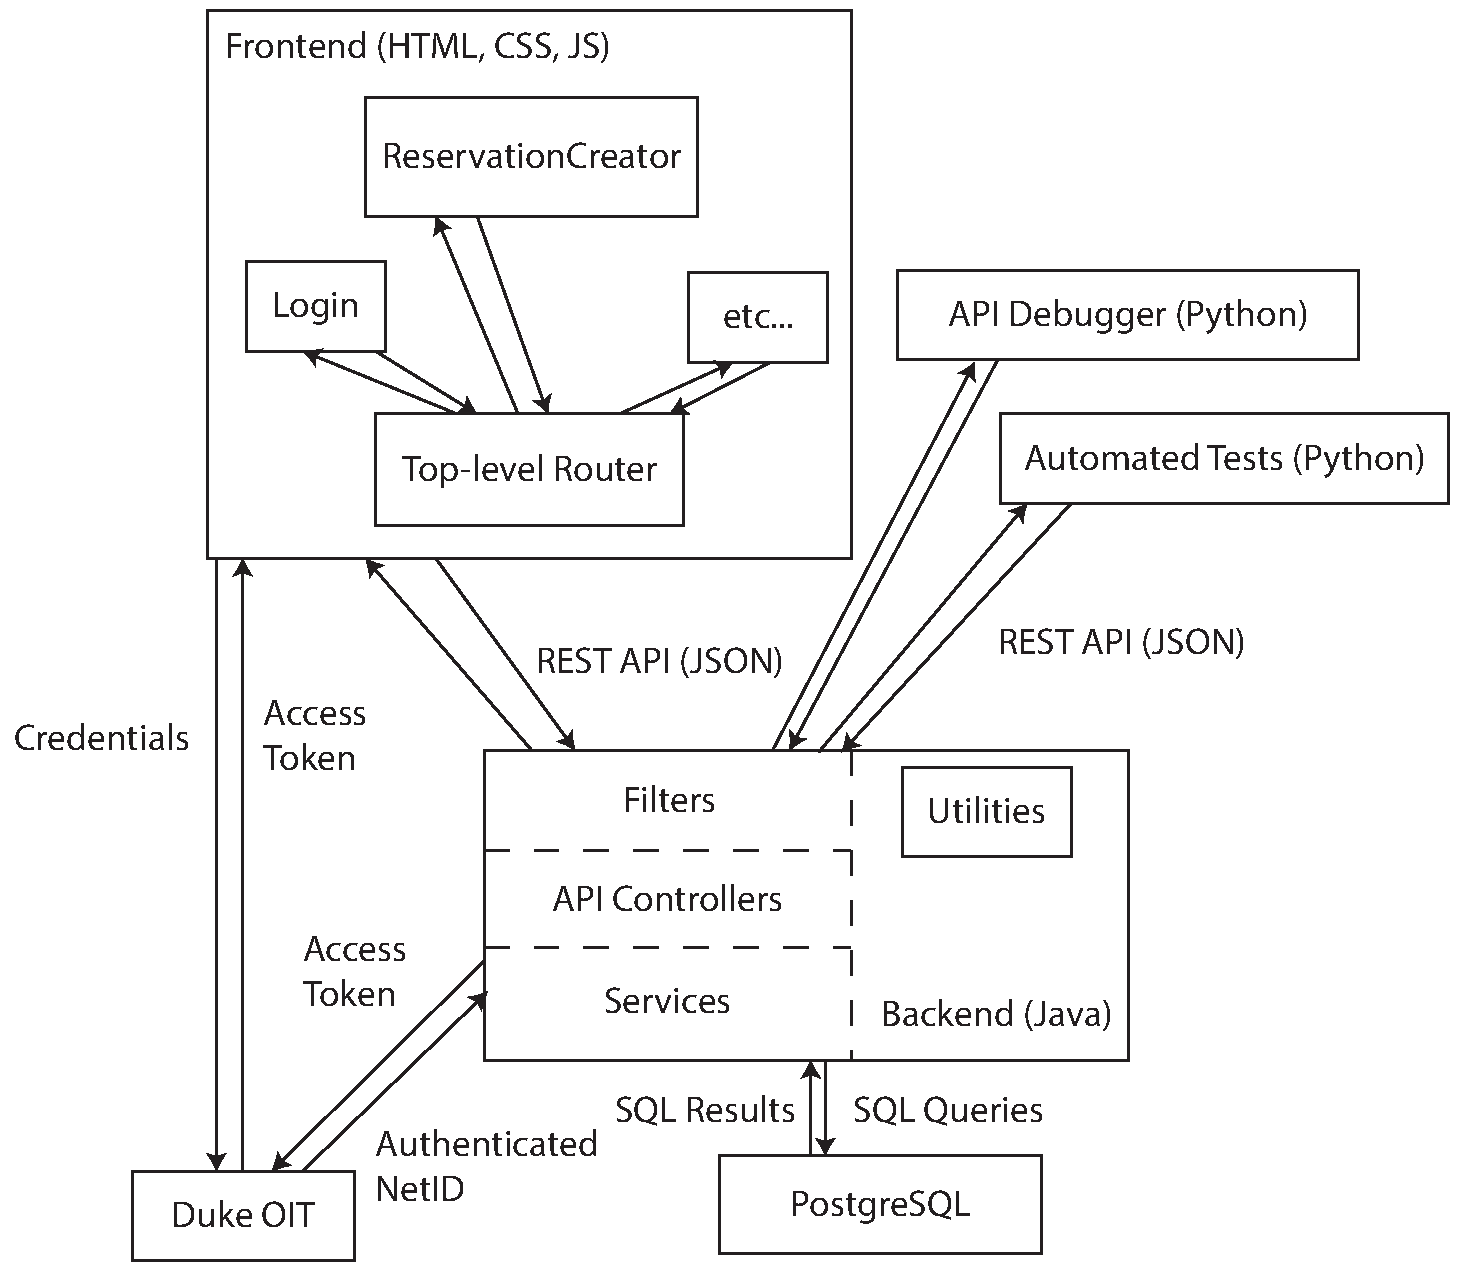
\includegraphics[height=4in]{ev2_design_cropped.pdf}
\end{center}
\caption{Diagram of system architecture}
\label{fig:design}
\end{figure}

Our resource management tool is a web application that uses the following technology stack: a React.js frontend, a Java Spring server, and a PostgreSQL database. In addition, we use Python scripts to automate the testing of our API. Our overall technology stack, as well as our overall code structure, have not changed since evolution 1. As can be seen in the diagram above, the two primary changes are:
\begin{enumerate}
    \item The inclusion of an API Debugger. This is just a python script that interacts with our backend, similarly to the way our python API tests function. 
    \item The inclusion of OAuth2 to handle duke net-id based authentication.
\end{enumerate}

The rest of the changes required for evolution 2 fit nicely into our existing frameworks. In the backend, permissions were handled with a few new API calls on top of our evolution 1 API calls, and a few new DB tables were added to support these calls. Similarly, groups were implemented via the addition of another controller and service. In the frontend, new views for permissions and groups were added.  

For retrospectives on our former backend choices and more detail about our backend additions, see the \hyperref[sec:Backend]{backend section}. For retrospectives on our former frontend choices and more detail about our frontend additions, see the \hyperref[sec:Frontend]{frontend section}. Finally, see \hyperref[appendix:backendtest]{Appendix \ref{appendix:backendtest}} for our updated backend test strategy,  \hyperref[appendix:frontendtest]{Appendix \ref{appendix:frontendtest}} for our updated frontend test strategy, \hyperref[appendix:apispec]{Appendix \ref{appendix:apispec}} for our updated API specification, and \hyperref[appendix:DBDesign]{Appendix \ref{appendix:DBDesign}} for our updated database design. 

\section{Backend}
\label{sec:Backend}
The backend consists of the parts of the software system that run on a VPS (Virtual Private Server) using Ubuntu Linux 14.04. Our software uses PostgreSQL 9.5 for persistent data storage and the Java Spring Framework as the container for a Tomcat web server. If the backend were viewed as an MVC (Model-View-Controller), PostgreSQL would be the model and Java Spring would be the view (REST API) and the controller (request processing, database communication, and response creation). 

This architecture has not changed since evolution 1, and it has suited as well. 

\subsection{Java}
\subsubsection{Retrospective}
At this point, we are quite content with our choice of Java as the backend language. Familiarity with Java has made development easy, and static typing has helped prevent bugs and improve code readability. Thus far, we have not encountered any problems that would have been much easier solved in another language. 

\subsubsection{Current Design}
Nothing has changed from a design perspective in terms of our choice of Java as a language. 

\subsection{Java Spring}
\subsubsection{Retrospective}
Spring has worked very well for us thus far. It is well documented, it has libraries for every use-case we have needed, and its MVC structure has made it easy to write our code in a maintainable way (for instance, adding a new set of endpoints for Groups was trivial - see the \hyperref[sec:GROUPS]{groups section}). We have had no significant issues with Spring so far. 

\subsubsection{Current Design}
Spring continues to be our backend framework, and thus nothing has changed from a design perspective in this regard.

\subsection{PostgreSQL}
\subsubsection{Retrospective}
PostgreSQL served us well for evolution 2. While perhaps more planning and setup was required for us to alter our DB schema from evolution 1 to evolution 2 than for a team using a NoSQL DB, we ultimately felt that this was a small amount of work. Furthermore, the result of such planning was a very clearly defined DB schema that made it easy for everyone (particurly those working on the backend) to understand how we were going to store data and therefore how to structure new endpoint code. Thus, we ultimately felt that having a structured DB improved our coding efficiency. 

In regards to choosing PostreSQL over some other SQL DB, we have not needed to interact with the DB in such a way that some other SQL DB would have provided us better tools than PostreSQL. Thus, we are still totally happy with PostreSQL as a DB. 

\subsubsection{Current Design}
The following changes were made to our DB schema for evolution 2:
\begin{enumerate}
    \item A Group table was added which tracks group settings and names. 
    \item A group members table was added. This tracks all the members of each group. 
    \item A user resource permissions table and a group resource permissions were added. These track resource permissions for each user and each group, respectively. 
    \item The user table was updated to include user permissions
\end{enumerate}

You can see a full diagram of this updated schema in  \hyperref[appendix:DBDesign]{Appendix \ref{appendix:DBDesign}}. 

\subsection{Security}
\subsubsection{Retrospective}
Our old security framework remained intact while tacking on Duke Shibboleth. We declined to use the tokens provided by Duke Shibboleth as they were undocumented and uncustomizable. 

\subsubsection{Current Design}
Evolution 2 introduced integration with Duke Shibboleth as a new requirement. We decided to keep our existing JSON web token (JWT) authentication framework and simply add Duke OAuth2 to our login. 

The evolution 2 spec requires that the old login stay intact for the admin, so we simply added a new button on the login page that redirected the user to a Duke-based authentication server. Depending on whether the user successfully authenticates using his or her NetID, the Duke server routes the user to a 'success' endpoint or a 'failure' endpoint. The failure endpoint is essentially the resource planner login page (with an added error message), while the success endpoint is a new endpoint which verifies the authcode returned by the Duke server using another Duke service. If this verification is successful, the user is logged in and given a JWT and directed to a page inside the resource manager. If this verification fails, the user is again redirected to the resource manager login. 

One major difference with the introduction of Duke Shibboleth authentication is the lack of user registration, since users can no longer be created by the admin. Instead, a user is 'created' the first time he or she logs into the resource planner. Besides the hashing and salting of the admin password, there is also no more password storage in our database as the resource planner no longer handles authentication directly, instead allowing Duke Shibboleth to simply pass us to an authcode after a successful user login that we can verify to ensure the user is valid. 

Upon login, a JSON Web Token (JWT) is generated, which stores the User ID and permission level of the logged-in user. This JWT, which is signed by a secret key known only to the server, authenticates future API calls without accessing the database. Instead of a database lookup, the authenticity of the JWT is confirmed using the secret key, and the User ID and permissions stored in the JWT can be used directly. 

For encrypting the communication between the client and the server, we decided to go with SSL as Spring provided support for it. We used Java's built in keytool to generate a Java keystore and self-signed certificate using RSA algorithm. We used a self-signed certificate rather than one signed by a legitimate CA because it was free. We also made it so that it can run on both HTTP and HTTPS at the same time for ease of testing. Non-SSL HTTP support can easily be disabled with a global switch.


\subsection{Testing}
\subsubsection{Retrospective}
For evolution 1 backend testing, we used a suite of API tests ran from a series of python scripts. This strategy worked extremely well for us - by having a set of tests which covered the vast majority of API cases, we could quickly make changes and verify that nothing was broken. We stand by our decision to focus on testing only the API contract, and not the backend internals, because ultimately the API is what must be working for the web application to work correctly. Realistically, any major bug in the internals of the backend should affect the API tests as well.


Now, there as some exceptions to this. For instance, email is be very hard to test via python scripts, and so our testing suite does not fully cover email. Similarly, since it is nearly impossible for an API testing suite to be 100 percent comprehensive, there are potentially situations where a backend bug would not break any tests, but would affect the web application. Nevertheless, we feel the chances of such issues ocurring is so low that they are not worth worrying about. Given the fact that our presentation for evolution 1 had no issues and that our evolution 1 passed all grader test cases, we still feel quite confident in this strategy. 

We also stand by our decision to use Python, as Python scripts are simple to write and can be run quickly. In addition, our Python testing framework  \texttt{unittest} has proven very easy to use, and Python has numerous libraries that allow you to easily send HTTP requests. 

\subsubsection{Current Design}
For evolution 2, we simply expanded our suite of tests to include groups, permissions, and the new login protocol with net-ids. These can be found in the classes test_AuthorizationTestCases.py, test_GroupsTestCases.py, and test_PermissionsTestCases.py. See (\hyperref[appendix:backendtest]{Appendix \ref{appendix:backendtest}}) for the full suite of tests. 

\subsection{Code Structure}
\subsubsection{Retrospective}
Our code structure went through a large, though simple refactoring. For evolution 1, we had all our backend code divided into filters, controllers, services, and utilities. This led to some issues where when a change was made in a controller, you would have to locate the corresponding service and make changes there. 
\subsubsection{Current Design}
For evolution 2, we decided to stay with a type of MVC. All backend code is either part of a utility, a 'module' or 'main'. The utility code remained essentially unchanged from evolution 1. A module is a package consisting of a controller, one or more services that serve that controller, and models that serve I/O or storage functions. For example, a group module has a group-controller which specifies the endpoints, a service module which performs the actions required for the requests send to the service from the endpoints, and a number of request and response object formats (models). Main essentially consists of non-utility code that is used across modules, such as filters and email services. 

This design allowed us to make changes to a module much more quickly, as we didn't have to look through other modules to find the specific module we wanted to modify. This further compartmentalization of our code allows us to retain a MVC design, albeit a module-based MVC rather than a backend-based MVC. This change made the already easy-to-use design even more intuitive and efficient. The new design is as extensible, if not more so than before. 

\subsection{Groups}
\label{sec:GROUPS}
\subsubsection{Current Design}
Groups are a new evolution 2 feature. Our implementation allows for two groups to have the same name (though they are unique as they have different IDs). A group is affiliated with zero or more members and the three types of system-wide permissions - resource permission, reservation permission, and user permission. The users with user permission have the ability to create groups, edit groups, edit group membership, and delete groups. 

There were not any particularly complex or challenging design decisions to make when implementing groups. From a database perspective, using one table for group settings and one table for group members is the most logical implementation. From a functionality perspective, the evolution 2 specification was very clear in what a group is. Finally, from a code perspective, we simply added another Controller and Service pair for groups, and its implementation very closely mimicked the UserController and UserService classes. This further demonsrates how well Spring and an MVC backend have worked for us. 


\subsection{Permissions}
\subsubsection{Current Design}
We debated heavily how to handle permissions for evolution 2. The largest question was whether to add a full set of permission endpoints to allow the frontend to query and modify specific permissions, or to consolidate permission editing and querying into a single call and thus a single view on the frontend. To clarify, the former case would involve numerous endpoints like GET /userResourcePermissions/\{user\_id\}, GET /groupSystemPermissions/\{group\_id\}, etc. whereas the latter would involve a single endpoint that would return a table of all permissions. 

The benefits of the former case include:
\begin{enumerate}
    \item More 'extensibility' in the sense that future requirements may further change how permissions work. In such a case, it may be better to have a number of discretized permission endpoints, rather than all permissions lumped into a single endpoint. 
    \item A less monolithic permission frontend. Multiple endpoints allow, for instance, one view for group system permissions, one view to edit the permissions for a resource, etc. 
\end{enumerate}

That being said, we ended up choosing to do the latter case, and the primary reason was simplicity. We have a single location where a user can edit all permissions on the front-end, we have a single API endpoint to query for all permissions that a user can change, and we have a single API endpoint to alter all permissions that a user can change. Doing things this way prevented us from having to alter every piece of the UI on the frontend, and also allowed us to consolidate permission code nicely in the backend. In addition, we feel it actually makes for a very nice user experience - the user always knows precisely where to go to change permissions. 

In addition, this strategy is still extensible in the sense that we can always easily add new permissions to this single permission manager table very easily. As such, we argue that this strategy is actually more extensible than the multiple endpoint strategy for future permission changes that are not radically different from current permission behavior. The multiple endpoint strategy would have to modify a lot of front-end code to adapt, whereas we could change almost nothing on the frontend. 

The downside, however, is that we are less capable of adapting to radically different permission guidelines. However, we feel this is a risk worth taking for now. 

\subsubsection{Assumptions}
Given the ambiguity of some of the permission guidelines, we want to outline our assumptions for permission behavior:
\begin{enumerate}
    \item The admin always has full permissions on everything. This can never be changed. 
    \item A new user or new group will, by default, have no system permissions. A user with user system permissions will need to go in and give them permissions. 
    \item A newly created resource defaults to VIEW permission for the user that created it, and no permission for all other users and groups. 
    \item A user with reservation management permissions can modify ANY reservation, including reservations for resources that the user does not himself have view or reserve access for. That being said, a user with reservation management permissions can not break any permission constraints when modifying a reservation (as an example, a user with reservation management permissions could not edit a reservation such that the edited reservation pairs a user with a resource that user does not have reserve access for). 
\end{enumerate}



\section{REST API}
\label{sec:REST}
Communication between the frontend and the backend is done through a REST API with JSON (\hyperref[appendix:apispec]{Appendix \ref{appendix:apispec}}).

\subsection{Retrospective}
The JSON-based REST API served us well for Evolution 2. We identified several strengths that helped us implement the new set of requirements: the well-understood nature of JSON and the fairly rich state transfer afforded to us. Furthermore, the weaknesses we identified (that the client must initiate all data transfer and JSON's rigid tree-of-values structure) did not affect us much when implemented Evolution 2.

One unexpected strength of our REST API was the requirement in Evolution 2 of having an API. In the early stages of the project, we were debating between server-side rendering and client-side rendering. Server-side rendering (e.g. Ruby on Rails) involves the server performing virtually all of the business logic and sending to the client fairly static HTML pages. Each time the user performs an action, he/she is taken to a new page that is rendered from scratch. By contrast, client-side rendering sees the user download a client application, which then executes API calls against the backend and updates the view. We chose to implement client-side rendering because it enables quicker UI updates (because typical REST API payloads are much smaller than typical webpages), but we did not anticipate the additional benefit that having a well-defined API meant that we could externalize the API when Evolution 2 asked us to.

\subsection{Current Design}
We expanded the set of endpoints that were required to implement the requirements in Evolution 2. Endpoints for creating, updating, and deleting groups were virtually identical to endpoints we had already written, so completing the groups feature went quickly. Endpoints for updating permissions was also similar to previous work. The slightly more complicated endpoints were those involved in OAuth authentication. Even then, the complexity was inherent to any OAuth implementation and we were not hindered by our previous design choice of a RESTful JSON API.

\section{Frontend}
\label{sec:Frontend}
The frontend consists of the parts of the software system that are transferred to the user's computer and are run in the user's browser. The officially supported browser is the latest version of Google Chrome, but other modern browsers should work as well. We use the third-party libraries React.js, Bootstrap, and JQuery, but React.js has the most implications for the code design.

\subsection{React.js}
\subsubsection{Retrospective}
The frontend is written in React.js, a library written at Facebook for building user interfaces (UIs). We have been pleased with React.js. Our only complaint has been that React.js has occasionally required somewhat large amounts of boilerplate. We have read online that this boilerplate can be significantly reduced with some more advanced React.js techniques like mix-ins. We plan to take advantage of this in future React.js projects, but for now the cost of updating the code to use mix-ins would be higher than the benefit of more concise code.

As we discussed in our Evolution 1 writeup, using React.js allows us to trivially avoid inconsistent UIs, since the view is re-rendered from the whole state. As expected, we did not encounter a single UI bug due displaying inconsistent data.

\subsubsection{Current Design}
We made no changes to our usage of React.js, as we were quite pleased with it.

\subsection{React components}
\subsubsection{Retrospective}
Within the React framework, we designed components to express the desired UI in a natural way. At the top level of the HTML body is a Router component. This Router's state includes a route and other state to mediate communication between views. The route is a string that indicates which part of the application the user is in (e.g. ``reservation\_list'').

The Router, depending on its route state, will render another component (e.g. Login, AdminConsole, ReservationList, GroupManager). All of these views are themselves just HTML renderings of their state. Each of these subcomponents contains their own state. We considered having a global datastore of resources and reservations, but decided that the simplest way to maintain correctness across views was to simply redownload the data each time.

This design served us well. One minor issue we encountered was related to sending information between components. Because the components rendered by the Router do not have knowledge about eachother, they must send information through the Router, which then passes the information as a 'prop' to the receiving subcomponent . Though this has worked well in practice, it does seem a bit unwieldy.

\subsubsection{Current Design}
For the new requirements in Evolution 2, we added a GroupManager component and a PermissionsManager component. We also made minor modifications to some of the other components built for Evolution 1. Because the components were completely separate, this task did not take long and we did not encounter any unexpected challenges. We are therefore quite pleased with our design, since it appears to conform to the open-closed principle.

\subsection{Testing}
\subsubsection{Retrospective}
For frontend testing, we decided to write a test plan (\hyperref[appendix:frontendtest]{Appendix \ref{appendix:frontendtest}}) that is intended to be performed manually. Testers can load the application and execute actions that are intended to exercise most of the code paths in the application. This manual testing has the advantage that it has a low upfront cost and it is easy to implement. The disadvantage is that it is slow and takes a lot of human time and energy.

One alternative is to perform automated UI testing. We are aware of two different types automated UI testing: 1) programmatic access to the application and 2) simulation of mouse/keyboard events and screenshots. We decided against 1) because the UI is still in an infantile stage, and the intended DOM changes quite frequently. We decided that programmatically testing for the presence of, say, a certain <div> tag would be prohibitively expensive. We decided against 2) for the same reason that the intended DOM changes quite frequently, but also because we decided that such an approach seemed very fragile.

We were very pleased with our decision not to implement automated UI testing. While we did encounter some UI bugs, these bugs did not take long enough to catch that they would have justified the significant cost of implementing automated UI testing. (It's important to note that automated UI testing only decreases the amount of time it takes to catch bugs, not the amount of time it takes to fix them, a process which is more properly called \emph{debugging}.)

\subsubsection{Current Design}
As a result of our success with the manual UI testing from evolution 1, the only changes to our methodology here are to increase the number of test cases to account for the new functionality introduced by the Evolution 2 requirements (TODO add testcases to appendix).

\section{Member contributions}
Kevin Do maintained the frontend, advocated for the frontend's needs in discussions with the backend team, and implemented the permissions manager.

Davis Treybig implemented much of the permission-related code, including new permission endpoints and permission-based checks for other API endpoints. 

Jiawei Zhang integrated Duke OAuth2 and implemented the group endpoints and system-wide permissions for users and groups.

Michael Han wrote and maintained the automated backend tests, and he also implemented the group manager UI TODO.

\clearpage
\appendix
\section{Backend Test Plan}
\label{appendix:backendtest}
\begin{enumerate}
	\item Authorization Tests
	\begin{enumerate}
		\item Registering a valid user
		\item Registering an invalid user with preexisting email
		\item Registering an invalid user without a password
		\item Logging in as valid user
		\item Logging in with wrong password
		\item Logging in with wrong email, correct username and password
		\item Logging in with wrong username, correct email and password
	\end{enumerate}
	\item Resource Tests
	\begin{enumerate}
		\item Create valid resource with no tags
		\item Create valid resource with tags
		\item Create invalid resource with no name
		\item Create valid resource with no description 
		\item Get resource with valid ID
		\item Get resource with invalid ID
		\item Get resources with valid query
		\item Get resources with query with non existing tags
		\item Put resource with valid ID with all fields updated
		\item Put resource with valid ID no fields updated
		\item Put resource with invalid ID
		\item Delete resource with valid ID
		\item Delete resource with invalid ID
		\item Get resources canDelete with valid ID
		\item Get resources canDelete with invalid ID
	\end{enumerate}
	\item Reservation Tests
	\begin{enumerate}
		\item Create valid reservation with valid user ID
		\item Create valid reservation with invalid user ID
		\item Create reservation with touching time intervals
		\item Create invalid reservation with invalid resource ID
		\item Create invalid reservation with invalid time range
		\item Get reservation with valid ID
		\item Get reservation with invalid ID
		\item Get reservation with valid query with resource and user lists
		\item Get reservation with valid query with valid time range
		\item Get reservation with valid query with invalid time range
		\item Put reservation with valid ID update all fields
		\item Put reservation with valid ID update no fields
		\item Put reservation with invalid ID
		\item Delete reservation with valid ID
		\item Delete reservation with invalid ID
	\end{enumerate}
	\item Tags Tests
	\begin{enumerate}
		\item Get all tags
	\end{enumerate}
	\item User Tests
	\begin{enumerate}
		\item Check only admin can create users
		\item Check that non admin cannot create users
		\item Create invalid user with preexisting username
		\item Create invalid user with preexisting email 
		\item Get user with valid ID
		\item Get user with invalid ID
		\item Put User with invalid ID
		\item Put user not as admin
		\item Delete user with valid ID
		\item Delete user with invalid ID
	\end{enumerate}
\end{enumerate}

\clearpage
\section{Frontend Test Plan}
\label{appendix:frontendtest}
\begin{enumerate}
	\item Login
	\begin{enumerate}
		\item Logging in as the admin works
		\item Logging in as a normal user works
		\item Entering the wrong credentials -> useful message
	\end{enumerate}
	\item Navbar
	\begin{enumerate}
		\item Resources -> resources list
		\item Reservations -> reservations list
		\item Admin console works
		\item Log out works
	\end{enumerate}
	\item Reservations List
	\begin{enumerate}
		\item Start+end can correctly filter reservations shown
		\item Tags can correctly filter reservations shown
		\item Can properly go to the ``New reservation'' view
		\item Can properly go to the ``Edit reservation'' view
		\item Normal user can delete reservations own reservations
		\item Normal user can NOT delete others' reservations
		\item Admin can delete any reservation
	\end{enumerate}
	\item Resources list
	\begin{enumerate}
		\item Tags can correctly filter resources shown
		\item Can properly go to the ``New resource'' view
		\item Normal user can not edit/delete anything
		\item Admin user can edit/delete anything
		\item Deleting a resource with a future reservation shows a warning
	\end{enumerate}
	\item New resource
	\begin{enumerate}
		\item Admin can make new resource
		\item Normal user can't make new resource
		\item Displays error messages when invalid
	\end{enumerate}
	\item New reservation
	\begin{enumerate}
		\item Normal user can make new reservation with their own user ID
		\item Normal user can't make new reservation with another user ID
		\item admin can make new reservation with any user ID
	\end{enumerate}
	\item Admin console
	\begin{enumerate}
		\item Admin can make new user
		\item Normal user can't make new user
	\end{enumerate}
\end{enumerate}

\clearpage
\section{API Specification}
\label{appendix:apispec}
\begin{enumerate}
\item POST /auth/register
Creates an account with specified email and password

Common errors: email taken

Returns a JSON object with is\_error (boolean), error\_msg (possibly empty string)

\item POST /auth/login
Logs into an account with specified email and password

Common errors: invalid email or password

Returns a JSON object with is\_error (boolean), error\_msg (possibly empty string). If is\_error is false, also returns the session token


\item POST /resources
Creates a resource with the specified name, description, and tags, and assigns it a new unique ID

Common errors: empty name

Returns a JSON object with is\_error (boolean), error\_msg (possibly empty string). If is\_error is false, also returns a resource subobject with all the fields that were actually committed (ideally, the same as the values that were passed in)

\item GET /resources/<ID>
Returns a JSON object with is\_error (boolean) and error\_msg (possibly empty string)

Common errors: Resource with the specified ID does not exist

If is\_error is false, also returns a ``resource'' subobject with all the fields of the resource with the supplied ID

\item GET /resources/
Runs the specified query on the set of all resources and returns those that match

Queries are specified by a URL parameters with a ``required\_tags'' object (list of strings) and ``excluded\_tags'' specifying the tags that the resources in the search results should all have

Returns a JSON object with is\_error (boolean) and error\_msg (possibly empty string)

If is\_error is false, also returns a ``resources'' subobject, a list of resources (including ID and all fields) that match the query

\item PUT /resources/<ID>
Updates a resource with the supplied ID. Only changes the supplied fields and leaves the rest alone

Returns a JSON object with is\_error (boolean), error\_msg (possibly empty string). If is\_error is false, also returns a resource subobject with all the fields that were actually committed (ideally, the same as the values that were passed in)

\item DELETE /resources/<ID>
Deletes the resource with the given ID, if it exists, AND deletes all associated reservations

Common error: resource with the specified ID does not exist

Returns a JSON object with is\_error (boolean) and error\_msg (possibly empty string)

\item POST /reservations
Creates a reservation with data specified by the payload's ``resource\_id'' (int), ``start\_timestamp'' (string), ``user\_id'' (int), and ``end\_timestamp'' (string), ``should\_email'' (boolean) fields and assigns it a new unique ID

Validates the user ID for the reservation based on the currently authenticated user

Returns a JSON object with is\_error (boolean), error\_msg (possibly empty string). If is\_error is false, also returns a reservation subobject with all the fields that were actually committed (ideally, the same as the values that were passed in)

\item GET /reservations/<ID>
Returns a JSON object with is\_error (boolean) and error\_msg (possibly empty string)

If is\_error is false, also returns a ``reservation'' subobject with all the fields of the resource with the supplied ID

\item GET /reservations/
Runs the specified query on the set of all reservations and returns those that match

Queries are specified by URL parameters with one or more of the following: ``resource\_ids'' field (list of ints) specifying the desired resource IDs of the reservations (ANY), ``user\_ids'' (list of ints) (ANY), ``start'' (string, ISO 8601), ``end'' (string, ISO 8601)

return anything that overlaps with time range. If no user\_ids or resource\_ids are specified, return ALL reservations in time range. 

Returns a JSON object with is\_error (boolean) and error\_msg (possibly empty string)

If is\_error is false, also returns a ``reservations'' subobject (list of objects), a list of reservations (including ID and all fields) that match the query, ``resources'' subobjects (list of resource objects used in reservations), and ``users'' subobject (list of users objects used in reservations)

\item PUT /reservations/<ID>
Updates a reservation with the supplied ID. Only changes the supplied fields and leaves the rest alone

Returns a JSON object with is\_error (boolean), error\_msg (possibly empty string). If is\_error is false, also returns a reservation subobject with all the fields that were actually committed (ideally, the same as the values that were passed in)

\item DELETE /reservations/<ID>
Deletes the reservation with the given ID, if it exists

Common error: no reservation with specified ID

Returns a JSON object with is\_error (boolean) and error\_msg (possibly empty string)


\item GET /tags
Returns a JSON object with ``tags'' (list of strings), a list of all tags

\item GET /resources/<ID>/canDelete
Returns whether future/current reservations exist relating to a resource, in order to see whether we want to delete. This should return true if and only if (any reservations overlap the current time or start after the current time).

Returns a JSON object with is\_error (boolean), error\_msg (possibly empty string). If is\_error is false, also returns a boolean ``can\_delete'' with the answer

\item POST /users
Creates a given user with data specified by the payload's ``email'' (string), ``password'' (string), ``username'' (string), ``should\_email'' (bool), A unique ID is automatically assigned by the DB. 

Error cases: must check that no user already exists with the given username. Must also verify that the admin is the one doing this (only admin can create users)

Returns a JSON object with is\_error (boolean), error\_msg (possibly empty string). If is\_error is false, also returns the user subobject that was created

\item GET /users/<ID>
Retrieves the user with a given ID, if such a user exists. 

Returns a JSON object with is\_error (boolean), error\_msg (possibly empty string). If is\_error is false, also returns the user subobject. 

\item PUT /users/<ID>
Updates a user with the supplied ID. Only changes the supplied fields and leaves the rest alone

Error Check: If username changes, must verify the new username is not already taken. Must also verify that the admin is the one doing this (only admin can modify users)

Returns a JSON object with is\_error (boolean), error\_msg (possibly empty string). If is\_error is false, also returns the full, updated user subobject. 

\item DELETE /users/<ID>
Deletes the user with the supplied ID. 

Error Check: verify that the user with the given ID exists

Returns a JSON object with is\_error (boolean) and error\_msg (possibly empty string)
\end{enumerate}

\clearpage
\section{DB Design}
{\huge TODO}
\label{appendix:DBDesign}


\end{document}